% !TEX root = mythesis.tex

%==============================================================================
\chapter{Mesonic Correlations}
\label{sec:signal}
%==============================================================================
% \newcommand{\todo}[1]{\textbf{\color{red}TODO: #1}}

In this section, we first provide the theoretical framework for computing two-point meson correlation functions on the lattice. We perform a study of the resulting mesonic correlator signal using various distillation parameters to determine the optimal parameters to use. In particular, we want to test the optimal size of the eigenvector basis used to generate our perambulators and elementals, as well as the number of source locations per configuration in order to obtain a good signal while keeping the computational cost contained. 

Wick's theorem says that a correlation function is given by the sum of all possible pairs of quark contractions, specifically batched tensor contractions \cite{Chen:2023zyy}. 
The meson mass spectrum is extracted via Bayesian analysis of two-point correlation functions. One can systematically improve the agreement with PDG values by using more statistics, employing a collection of ensembles with various quark mass values and lattice spacing. Ultimately, the continuum masses are what we are after. For the study of scattering processes, a Luescher Analysis can be performed in tandem with the spectrum calculations, forging a connection between lattice data and phenomenology. We will briefly walk through the Bayesian fitting approach to extract meson masses, the process by which the ``raw" correlator data is converted into the principal correlator, rotated correlator, or some chosen effective quantity in the optimized basis. 

\section{Basic Correlation Functions}
Given a dimeson operator $[MM']$, we have the following spectral decomposition: 
\begin{align}
    \braket{[MM'](t) [MM']^\dagger(0)} = \sum_{n}^{} |Z_{MM'}^{(n)}|^2 e^{-E_{MM'}^{(n)}t}
\end{align}

As described in \todo{operator section ref }, we can form a set of $N$ $MM'$ interpolating operators(interpolators) $$\{[MM']^{(0)},\dots,[MM']^{(N)}\}$$ which have non-trivial overlap with the mesonic state of interest $MM'$. The question is thus, How does one determine the magnitude of the overlaps with the state of interest? Conveniently, the outer product of the set of $N$ interpolating operators acting on itself creates a $N \times N$ matrix of $MM'$ correlators. Not surpisingly, these share the same spectrum. 

In theory, one could fit all $N \times N$ correlators using a simultaneous fit, however, at this point it is standard practice to solve the generalized eigenvalue problem for the set of correlation functions. Solving the following for the eigenvectors $v_n(t,t_0)$ gives us an optimized operator basis
\begin{align}
    C(t)v_n(t,t_0) = \lambda_n(t,t_0)C(t_0)v_n(t,t_0)
\end{align}
Instead of solving the GEVP at the operator level, we deal with the correlation functions directly to yield the optimized correlators 
\begin{align}
    \braket{[\mathbb{MM'}](t) [MM']^\dagger(0)} = \sum_{n}^{} |Z_{MM'}^{(n)}|^2 e^{-E_{MM'}^{(n)}t} 
\end{align}


$(\bar{\psi}^{f_1}(n)\Gamma\psi^{f_2}(n))^{\dagger} = \pm \bar{\psi}^{f_2} \Gamma \psi^{f_1}$
which can be derived from the fact that the interchange of grassmann variables induces a minus sign and the $\gamma_4$ appears via the relation $\bar{\psi} = \psi^{\dagger}\gamma_4$
TLDR; the conjugate interpolator is obtained by interchanging the $\psi$ and $\bar{\psi}$ and ordering the barred quark fields to the left. 

Now we actually have to evaluate the correlators by employing the property that the fermionic expectation value factorizes with respect to the flavors. We then apply wick's theorem for each of the two flavors, this is fermion contraction , by which we obtain the dirac operators. In this case, only grassmann variables with equal flavor can be contracted with eachother

\section{Pion correlator} 
iven an operator with pion quantum numbers, such as
\[
\phi_L(x) = \bar{d}(x)\gamma_5u(x)
\]
or some smeared version of this, denoted $\phi_S(x)$,
the dimensionless correlator from Euclidean time $t_i$ to Euclidean time $t_f$
with momentum $\vec p$ is
\begin{eqnarray}
\Gamma^{\pi\pi}_{AB}(t_i,t_f,\vec{p})
 &=& a^6\sum_{{\vec x}_f}e^{-i(\vec{x}_f-\vec{x}_i)\cdot\vec{p}}
     \left<0\left|\phi_B(x_f)\phi_A^\dagger(x_i)\right|0\right> \nonumber \\

\end{eqnarray}


\section{Mesonic Signal Saturation}

We present preliminary results for the mass and overlap factors of a single pion with $\vec{p} = (000)$ in order to determine the optimal distillation parameters eg. rank of the distillation basis and number of time sources. This determination will allow us to optimize compute resources for the eigenbasis, perambulators, and elementals for the rest of the ensembles \todo{see ensemble table} we have generated. 
\section{Correlator Fits}

Here we present results for a systematic study of how the signal of the pion two-point correlator with $\vec{p}=(0,0,0)$ is affected by the rank of the distillation basis (number of eigenvectors used) and the number of $t_{src}$ insertions. The sizes of the distillation basis take values in the set $n_{vec}\in {32,64,96,128}$ and the number of $t_{src} \in {1,2,4,8,12,24}$. We perform this study on the ensemble $\beta = 3.7$, $m_{ud}=-0.0220$, $m_s = -0.0$, $L^3 \times T = 32^3\times96$

The raw correlators after averaging over all $t_{src}$ \todo{insert plot of corrs from corrfit}

The effective masses for each $n_{vec}$: \todo{insert plot}


\subsubsection{$n_{vec}$ dependence}

\begin{figure}[h]
    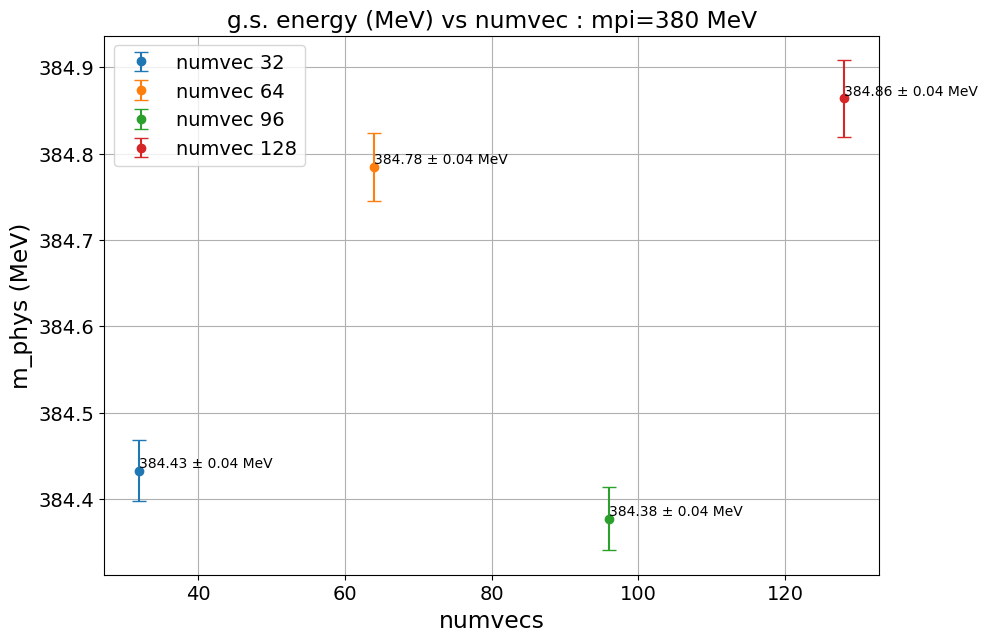
\includegraphics[width=1.0\textwidth, inner]{nvecs.png}
    \caption{comparison of ground state energy of the pion for different sizes(rank) of the distillation basis}
    \label{fig:figure2}
    \end{figure}

\subsubsection{$t_{src}$ dependence}
\begin{figure}[h]
    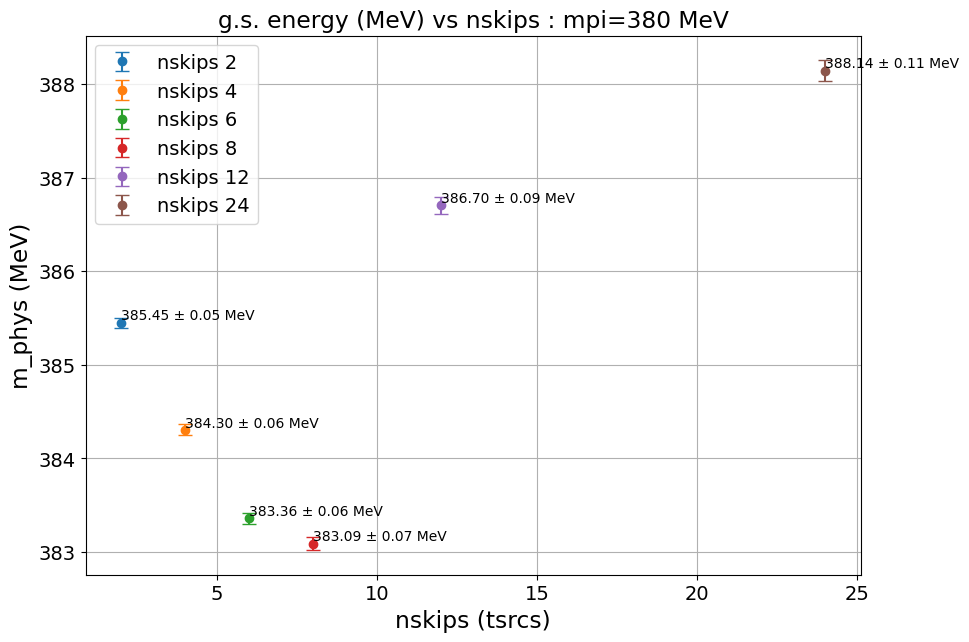
\includegraphics[width=1.0\textwidth, inner]{tsrc_nskips.png}
    \caption{comparison of ground state energy of the pion for various number of $t_{src}$ insertions}
    \label{fig:figure3}
    \end{figure}
\begin{figure}[h]
    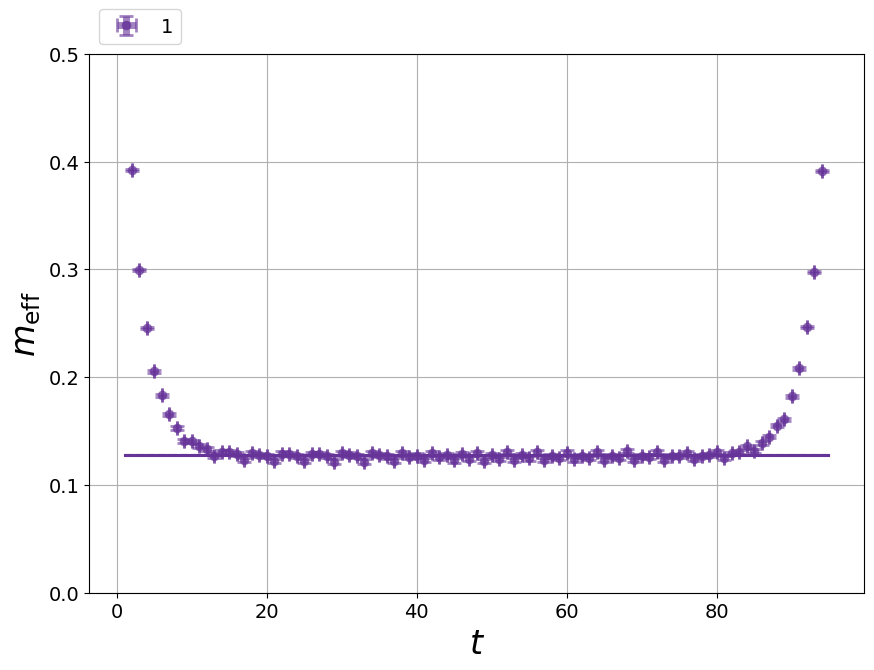
\includegraphics[width=1.0\textwidth, inner]{nskip_1.png}
    \caption{single state fit to the effective mass of the pion for 24 $t_{src}$ insertions}
    \label{fig:figure4}
    \end{figure}
    
We performed a systematic study of the mesonic signal saturation using the pion as a test case as it typically provies the cleanest signal in lattice calculations. With this complete, we will proceed with computing the fundamental distillation objects using a distillation basis of rank 96 and 24 $t_{src}$ insertions for the perambulators. 


\newpage

\section{Momentum projection}
For non-local operators used to construct mesons in flight, we must momentum project into states of definite momentum, which will reside in some irreducible representation of the octahedral group. 

We want hadrons tates to be states of definite spatial momentum $\textbf{p}$ 
$\tilde{O}(\textbf{p},n_t) = \frac{1}{\sqrt{\Lambda_3}} \sum_{n\in\Lambda_3} O(\textbf{n},nt)e^{-ia\textbf{np}}$ 

The interpolator is projected to definite spatial momentum and is located on a single time slice $n_t$

Note that it is only necessary to project one of the two interpolators of a correlation function to definite momentum, typically at the sink. 



